
\chapter{Statistical Analysis for the Antenna Benchmarks}\label{stat-ant}
\singlespacing
\vspace{-1cm}
\hypertarget{hypothesis-testing}{%A
\section{Tests and Hypotheses for the Statistical Analyses}\label{hypothesis-testing}}

\begin{enumerate}
\setlength{\itemsep}{0em}
\item Testing if the means are same with Welch Two Sample t-test
\begin{itemize} 
\setlength{\itemsep}{0em}
\item H0: True difference in means is equal to 0
\item H1: True difference in means is not equal to 0
\end{itemize} 
\item Testing if the data are coming from the same distribution with
Two-sample Kolmogorov-Smirnov test
\begin{itemize} 
\setlength{\itemsep}{0em}
\item H0: Two distributions are same
\item H1: Two distributions are not same
\end{itemize} 
\end{enumerate}




\section{Summary of the Benchmark Results}\label{bench-sum}

\renewcommand{\arraystretch}{1.2}%
\begin{table}[H]
\begin{center}
\caption{Reception Benchmark summary.}
\label{tab:rbs}
\begin{adjustbox}{max width=\textwidth}
\begin{tabular}{| l || c | c | c | c | c | c | c |}
\hline
\rowcolor{lightgray}
\textbf{Type} & \textbf{Count} & \textbf{Mean} & \textbf{SD}  & \textbf{Median} & \textbf{Min} & \textbf{Max}  & \textbf{IQR}\tabularnewline \hline \hline 
\cellcolor{lightgray} \textbf{Omni}     & 130 & 24.7313 & 1.3544 & 25.3 & 18.3 & 26.3 & 1.2 \tabularnewline \hline
\cellcolor{lightgray} \textbf{Directed} & 130 & 26.0618 & 2.2429 & 27.0 & 19.4 & 28.4 & 1.1 \tabularnewline \hline
\cellcolor{lightgray} \textbf{DirectedX} & 130 & 27.0435 & 1.6653 & 27.6 & 22.7 & 30.4 & 1.9 \tabularnewline \hline
\end{tabular}
\end{adjustbox}
\end{center}
\end{table}
\renewcommand{\arraystretch}{1}%



\renewcommand{\arraystretch}{1.2}%
\begin{table}[H]
\begin{center}
\caption{Transmission Benchmark summary.}
\label{tab:tbs}
\begin{adjustbox}{max width=\textwidth}
\begin{tabular}{| l || c | c | c | c | c | c | c |}
\hline
\rowcolor{lightgray}
\textbf{Type} & \textbf{Count} & \textbf{Mean} & \textbf{SD}  & \textbf{Median} & \textbf{Min} & \textbf{Max}  & \textbf{IQR}\tabularnewline \hline \hline 
\cellcolor{lightgray} \textbf{Omni}      & 130 & 44.8198 & 4.4378 & 41.9 & 36.5 & 57.0 & 5.2 \tabularnewline \hline
\cellcolor{lightgray} \textbf{Directed}  & 130 & 45.7252 & 4.4499 & 43.8 & 37.5 & 52.4 & 10.5 \tabularnewline \hline
\cellcolor{lightgray} \textbf{DirectedX} & 130 & 44.7481 & 4.3086 & 41.9 & 38.6 & 52.4 & 5.0 \tabularnewline \hline
\end{tabular}
\end{adjustbox}
\end{center}
\end{table}
\renewcommand{\arraystretch}{1}%



% 
% \hypertarget{statistical-analysis-for-the-reception-benchmark}{%
% \section{Statistical Analysis for the Reception
% Benchmark}\label{statistical-analysis-for-the-reception-benchmark}}
% \vspace{-0.5cm}
% \begin{longtable}[]{@{}cccccccc@{}}
% \caption{Reception Benchmark Summary}\tabularnewline
% \toprule
% Type & count & mean & sd & median & min & max & IQR\tabularnewline
% \midrule
% \endfirsthead
% \toprule
% Type & count & mean & sd & median & min & max & IQR\tabularnewline
% \midrule
% \endhead
% Directed & 131 & 26.0618 & 2.2429 & 27.0 & 19.4 & 28.4 &
% 1.1\tabularnewline
% DirectedX & 131 & 27.0435 & 1.6653 & 27.6 & 22.7 & 30.4 &
% 1.9\tabularnewline
% Omni & 131 & 24.7313 & 1.3544 & 25.3 & 18.3 & 26.3 & 1.2\tabularnewline
% \bottomrule
% \end{longtable}

% 
% \begin{figure}[!htbp]
%  \begin{center}
%   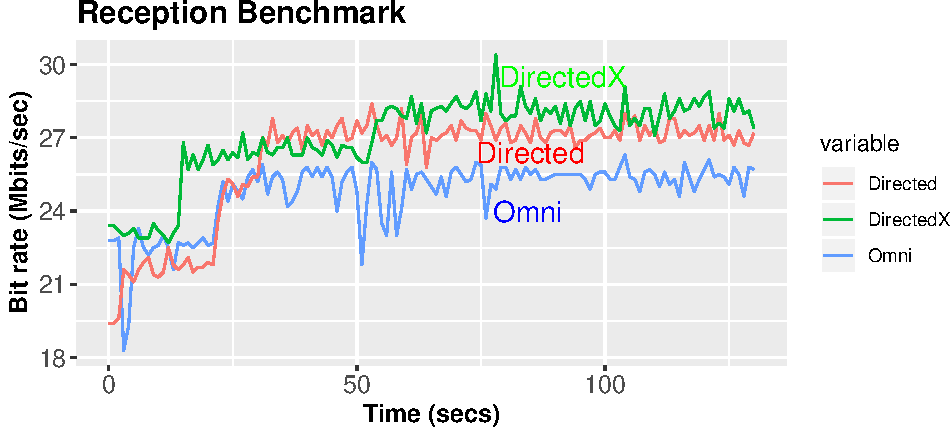
\includegraphics[width=\textwidth]{analyze1-1.pdf}
%  \end{center}
%  \caption{figure.}
%   \label{fig:cf1}
% \end{figure}


%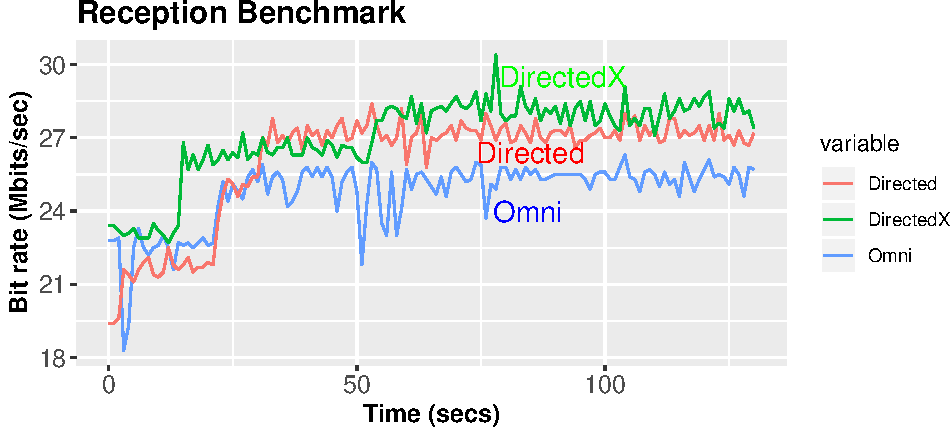
\includegraphics{analyze1-1.pdf}

\newpage




\section{Descriptive Plots of the Reception Data}\label{plot-reception}



\begin{figure}[!htbp]
 \begin{center}
  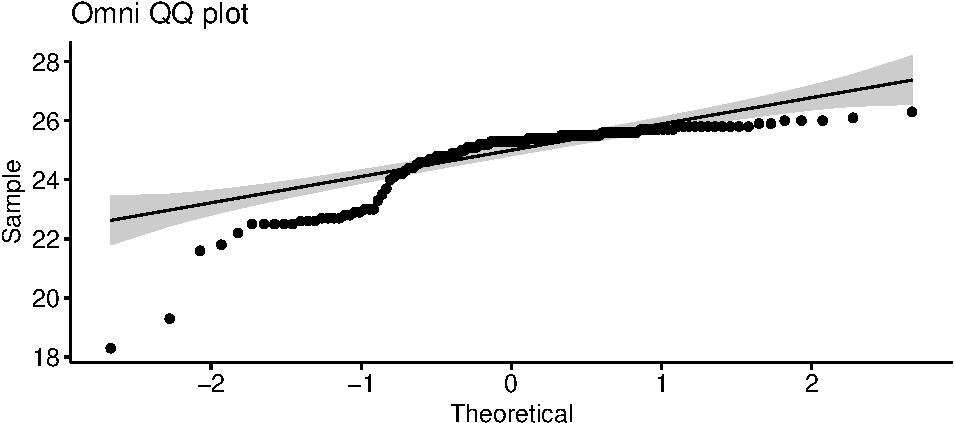
\includegraphics[width=0.85\textwidth]{analyze2-1.pdf}
 \end{center}
 \caption{QQ plot of the data rate observations for the Omnidirectional Antenna.}
  \label{fig:cf21}
\end{figure}

\begin{figure}[!htbp]
 \begin{center}
  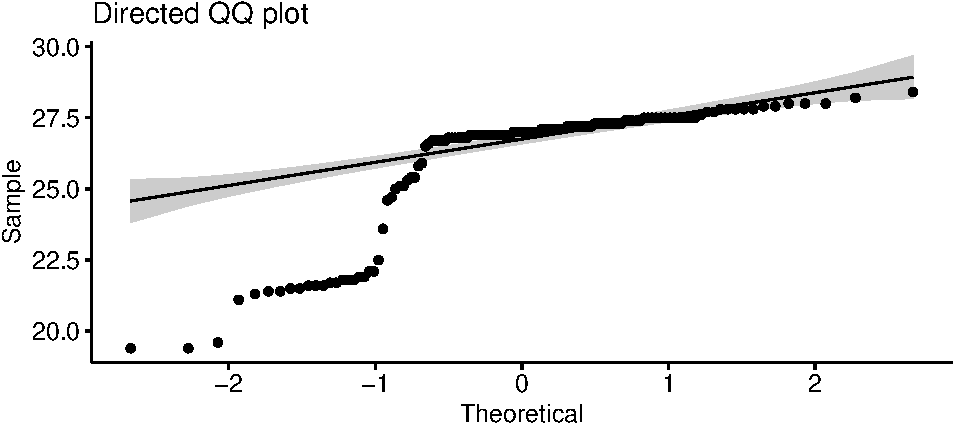
\includegraphics[width=0.85\textwidth]{analyze2-2.pdf}
 \end{center}
 \caption{QQ plot of the data rate observations for the Directional Antenna.}
  \label{fig:cf22}
\end{figure}

\begin{figure}[!htbp]
 \begin{center}
  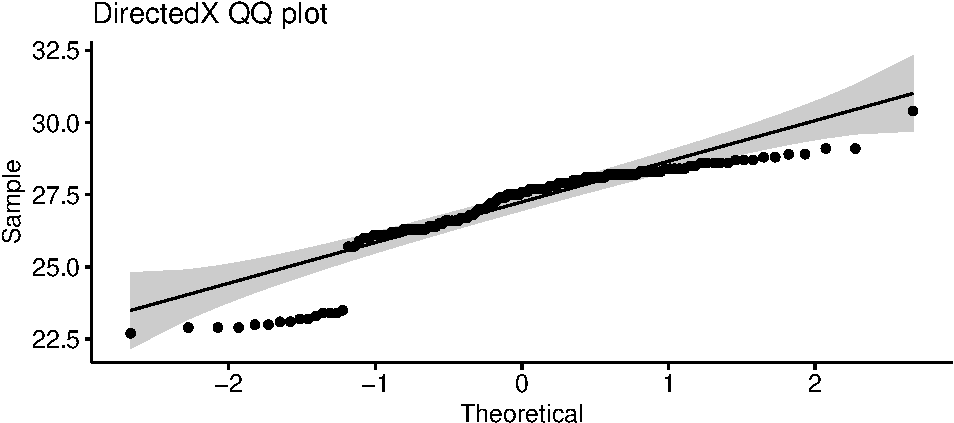
\includegraphics[width=0.85\textwidth]{analyze2-3.pdf}
 \end{center}
 \caption{QQ plot of the data rate observations for the Directional Antenna (tuned version).}
  \label{fig:cf23}
\end{figure}

\newpage



\begin{figure}[!htbp]
 \begin{center}
  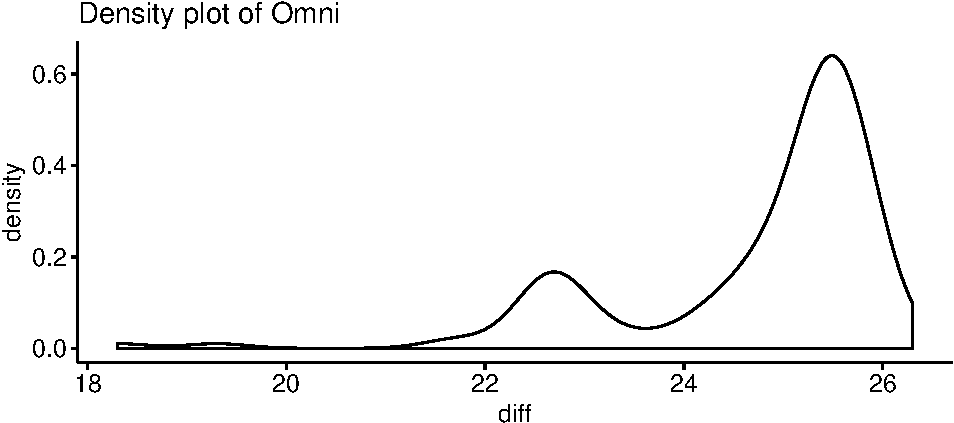
\includegraphics[width=0.85\textwidth]{analyze5-1.pdf}
 \end{center}
 \caption{Density plot of the data rate observations for the Omnidirectional Antenna.}
  \label{fig:cf51}
\end{figure}

\begin{figure}[!htbp]
 \begin{center}
  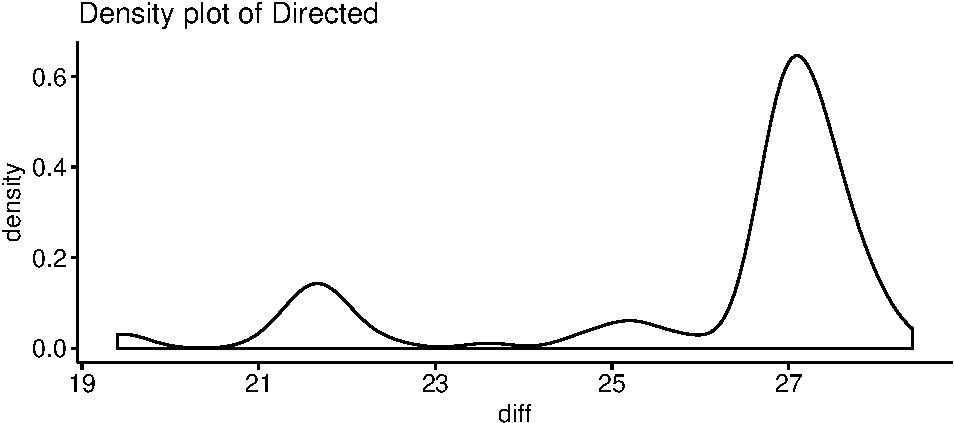
\includegraphics[width=0.85\textwidth]{analyze5-2.pdf}
 \end{center}
 \caption{Density plot of the data rate observations for the Directional Antenna.}
  \label{fig:cf52}
\end{figure}

\begin{figure}[!htbp]
 \begin{center}
  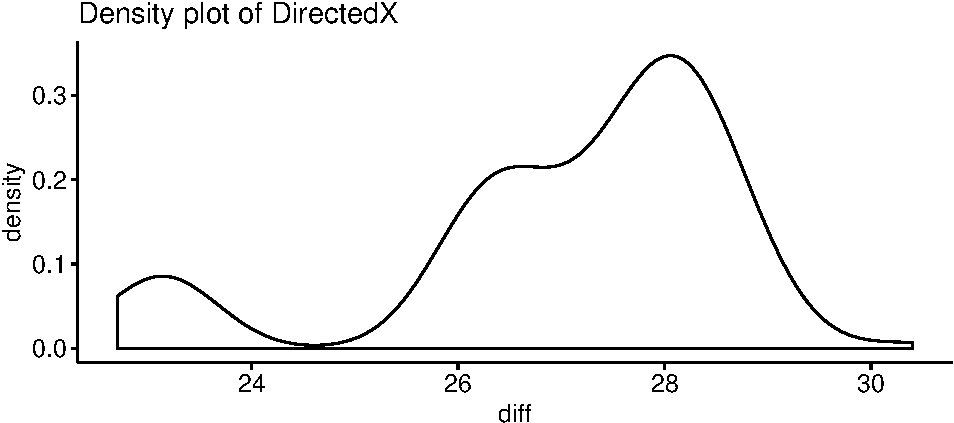
\includegraphics[width=0.85\textwidth]{analyze5-3.pdf}
 \end{center}
 \caption{Density plot of the data rate observations for the Directional Antenna (tuned version).}
  \label{fig:cf53}
\end{figure}

\newpage



\begin{figure}[!htbp]
 \begin{center}
  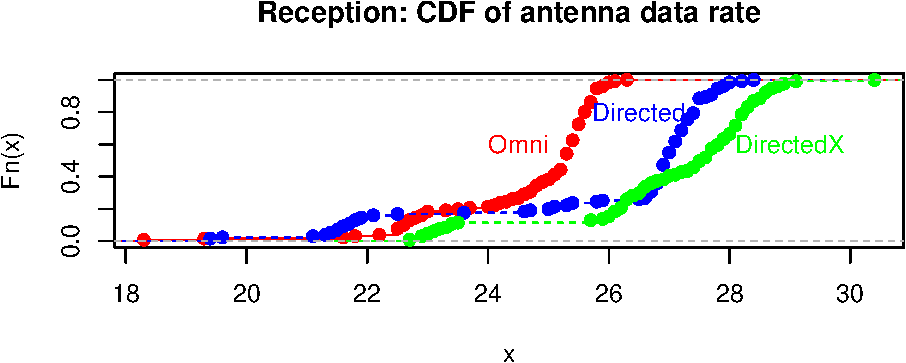
\includegraphics[width=0.85\textwidth]{analyze8-1.pdf}
 \end{center}
 \caption{Cumulative Distribution Function for the data rate observations.}
  \label{fig:cf81}
\end{figure}

\begin{figure}[!htbp]
 \begin{center}
  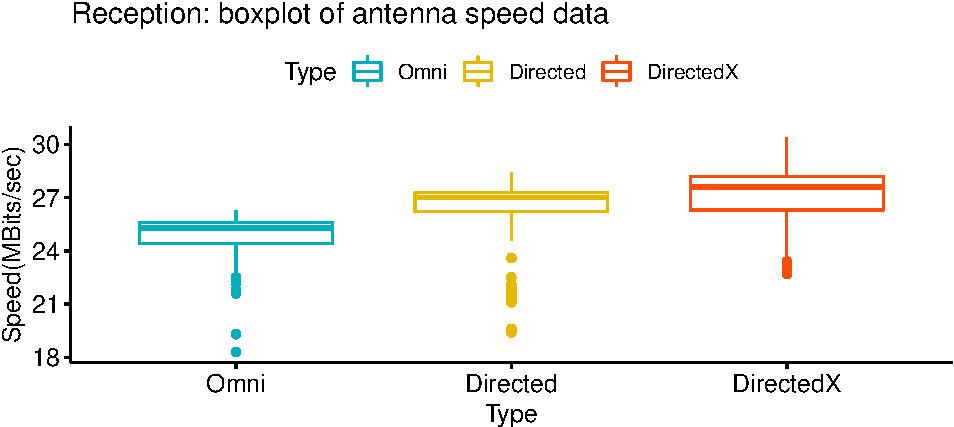
\includegraphics[width=0.85\textwidth]{analyze8-2.pdf}
 \end{center}
 \caption{Boxplot for the data rate observations.}
  \label{fig:cf82}
\end{figure}

\begin{figure}[!htbp]
 \begin{center}
  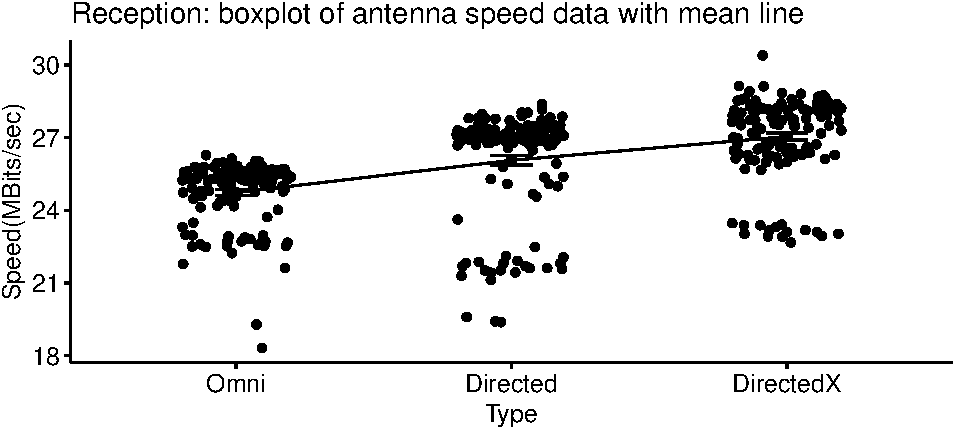
\includegraphics[width=0.85\textwidth]{analyze8-3.pdf}
 \end{center}
 \caption{Boxplot for the data rate observations with the mean line connected.}
  \label{fig:cf83}
\end{figure}

\newpage

\section{R Codes and Results for the Statistical Tests on the Reception Data}\label{rreception}
\begin{Shaded}
\begin{Highlighting}[]
\CommentTok{# Testing if the means are same with Welch Two Sample t-test}
\CommentTok{# H0: True difference in means is equal to 0}
\CommentTok{# H1: True difference in means is not equal to 0}
\CommentTok{# If the p-value of the test is less than the significance}
\CommentTok{# level alpha = 0.05.}
\CommentTok{# We reject the Null Hypothesis that: }
\CommentTok{# The means do not have statistically significant difference}
\KeywordTok{t.test}\NormalTok{(Omni,Directed, }\DataTypeTok{alternative =} \StringTok{"two.sided"}\NormalTok{)}
\end{Highlighting}
\end{Shaded}

\begin{verbatim}
##  Welch Two Sample t-test
## data:  Omni and Directed
## t = -5.8122, df = 213.69, p-value = 2.221e-08
## alternative hypothesis: true difference in means is not equal to 0
## 95 percent confidence interval:
##  -1.7817661 -0.8793026
## sample estimates:
## mean of x mean of y 
##  24.73130  26.06183
\end{verbatim}

\begin{Shaded}
\begin{Highlighting}[]
\KeywordTok{t.test}\NormalTok{(Directed,DirectedX, }\DataTypeTok{alternative =} \StringTok{"two.sided"}\NormalTok{)}
\end{Highlighting}
\end{Shaded}

\begin{verbatim}
##  Welch Two Sample t-test
## data:  Directed and DirectedX
## t = -4.0221, df = 239.93, p-value = 7.732e-05
## alternative hypothesis: true difference in means is not equal to 0
## 95 percent confidence interval:
##  -1.4624757 -0.5008831
## sample estimates:
## mean of x mean of y 
##  26.06183  27.04351
\end{verbatim}

\begin{Shaded}
\begin{Highlighting}[]
\KeywordTok{t.test}\NormalTok{(Omni,DirectedX, }\DataTypeTok{alternative =} \StringTok{"two.sided"}\NormalTok{)}
\end{Highlighting}
\end{Shaded}

\begin{verbatim}
##  Welch Two Sample t-test
## data:  Omni and DirectedX
## t = -12.329, df = 249.64, p-value < 2.2e-16
## alternative hypothesis: true difference in means is not equal to 0
## 95 percent confidence interval:
##  -2.681588 -1.942840
## sample estimates:
## mean of x mean of y 
##  24.73130  27.04351
\end{verbatim}

\pagebreak

\begin{Shaded}
\begin{Highlighting}[]
\CommentTok{# Testing if the data are coming from the same distribution with }
\CommentTok{# Two-sample Kolmogorov-Smirnov test}
\CommentTok{# H0: Two distributions are same}
\CommentTok{# H1: Two distributions are not same}
\CommentTok{# If the p-value of the test is less than the significance}
\CommentTok{# level alpha = 0.05.}
\CommentTok{# We reject the Null Hypothesis that two groups are coming} 
\CommentTok{# from the same dist.}
\KeywordTok{ks.test}\NormalTok{(Omni,Directed, }\DataTypeTok{alternative =} \StringTok{"two.sided"}\NormalTok{)}
\end{Highlighting}
\end{Shaded}
% 
% \begin{verbatim}
% ## Warning in ks.test(Omni, Directed, alternative = "two.sided"): p-value will
% ## be approximate in the presence of ties
% \end{verbatim}

\begin{verbatim}
## 
##  Two-sample Kolmogorov-Smirnov test
## 
## data:  Omni and Directed
## D = 0.74809, p-value < 2.2e-16
## alternative hypothesis: two-sided
\end{verbatim}

\begin{Shaded}
\begin{Highlighting}[]
\KeywordTok{ks.test}\NormalTok{(Directed,DirectedX, }\DataTypeTok{alternative =} \StringTok{"two.sided"}\NormalTok{)}
\end{Highlighting}
\end{Shaded}
% 
% \begin{verbatim}
% ## Warning in ks.test(Directed, DirectedX, alternative = "two.sided"): p-value
% ## will be approximate in the presence of ties
% \end{verbatim}

\begin{verbatim}
## 
##  Two-sample Kolmogorov-Smirnov test
## 
## data:  Directed and DirectedX
## D = 0.38931, p-value = 4.766e-09
## alternative hypothesis: two-sided
\end{verbatim}

\begin{Shaded}
\begin{Highlighting}[]
\KeywordTok{ks.test}\NormalTok{(Omni,DirectedX, }\DataTypeTok{alternative =} \StringTok{"two.sided"}\NormalTok{)}
\end{Highlighting}
\end{Shaded}
% 
% \begin{verbatim}
% ## Warning in ks.test(Omni, DirectedX, alternative = "two.sided"): p-value
% ## will be approximate in the presence of ties
% \end{verbatim}

\begin{verbatim}
## 
##  Two-sample Kolmogorov-Smirnov test
## 
## data:  Omni and DirectedX
## D = 0.83206, p-value < 2.2e-16
## alternative hypothesis: two-sided
\end{verbatim}

\pagebreak


\section{Descriptive Plots on the Transmission Data}\label{plot-trans}



% 
% \begin{longtable}[]{@{}cccccccc@{}}
% \caption{Transmission Benchmark Summary}\tabularnewline
% \toprule
% Type & count & mean & sd & median & min & max & IQR\tabularnewline
% \midrule
% \endfirsthead
% \toprule
% Type & count & mean & sd & median & min & max & IQR\tabularnewline
% \midrule
% \endhead
% Directed & 131 & 45.7252 & 4.4499 & 43.8 & 37.5 & 52.4 &
% 10.5\tabularnewline
% DirectedX & 131 & 44.7481 & 4.3086 & 41.9 & 38.6 & 52.4 &
% 5.0\tabularnewline
% Omni & 131 & 44.8198 & 4.4378 & 41.9 & 36.5 & 57.0 & 5.2\tabularnewline
% \bottomrule
% \end{longtable}

%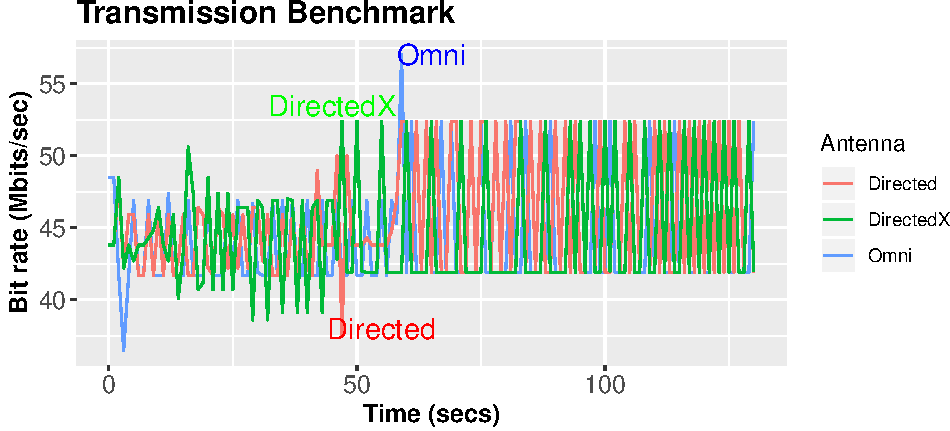
\includegraphics{analyze19-1.pdf}


% 
% 
% 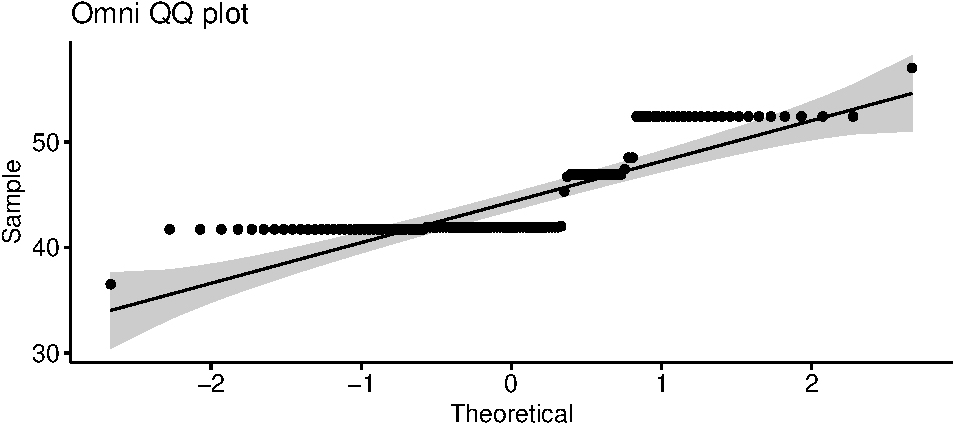
\includegraphics{analyze20-1.pdf}
% 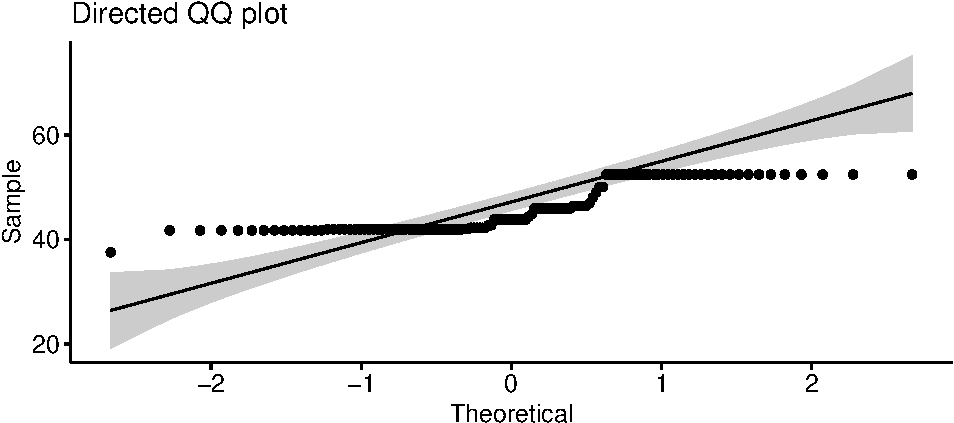
\includegraphics{analyze20-2.pdf}
% 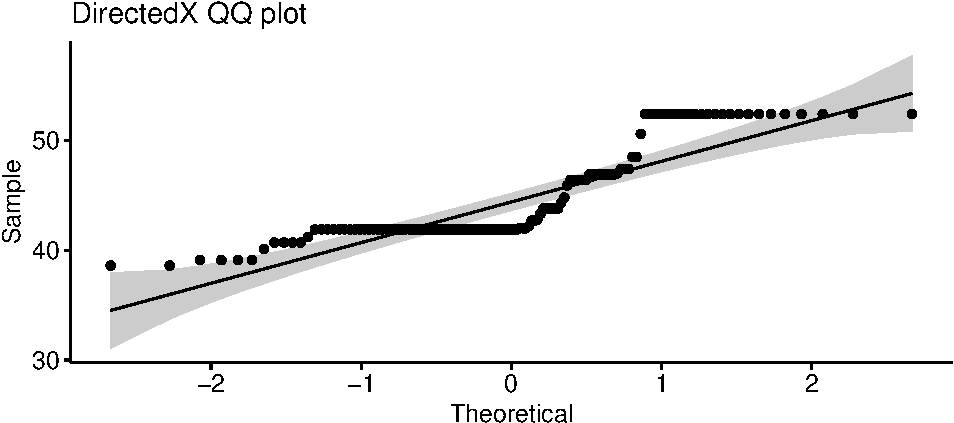
\includegraphics{analyze20-3.pdf}


\begin{figure}[!htbp]
 \begin{center}
  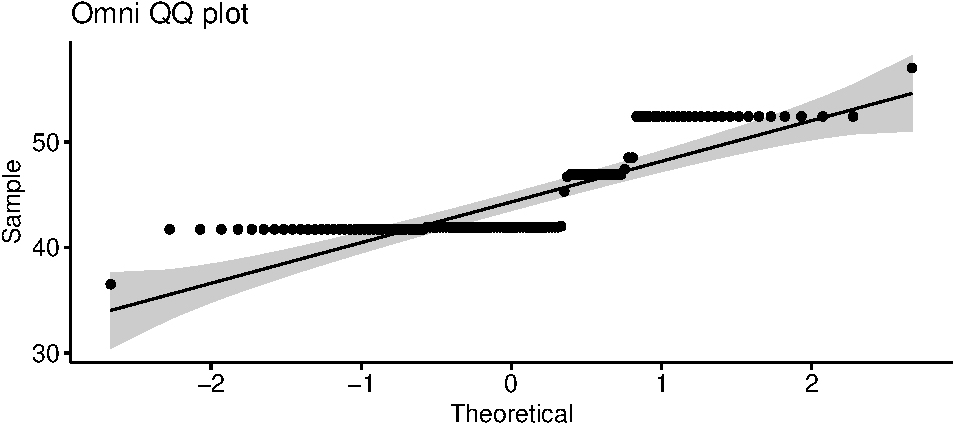
\includegraphics[width=0.85\textwidth]{analyze20-1.pdf}
 \end{center}
 \caption{QQ plot of the data rate observations for the Omnidirectional Antenna.}
  \label{fig:cf201}
\end{figure}

\begin{figure}[!htbp]
 \begin{center}
  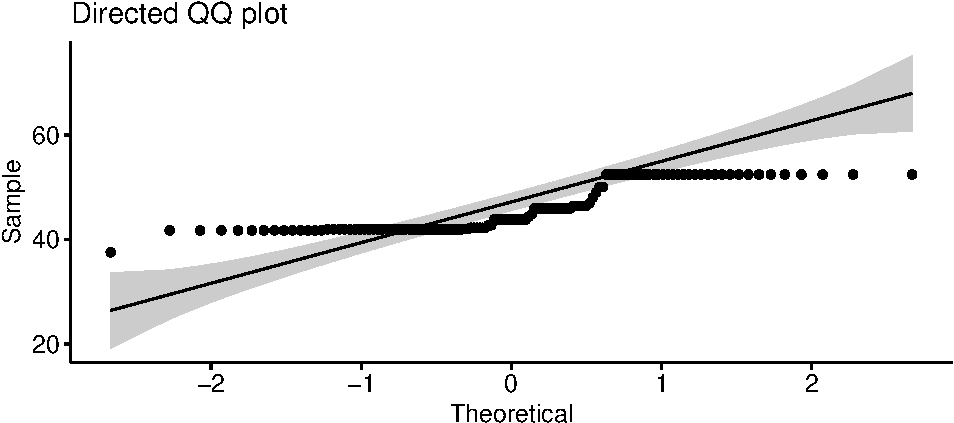
\includegraphics[width=0.85\textwidth]{analyze20-2.pdf}
 \end{center}
 \caption{QQ plot of the data rate observations for the Directional Antenna.}
  \label{fig:cf202}
\end{figure}

\begin{figure}[!htbp]
 \begin{center}
  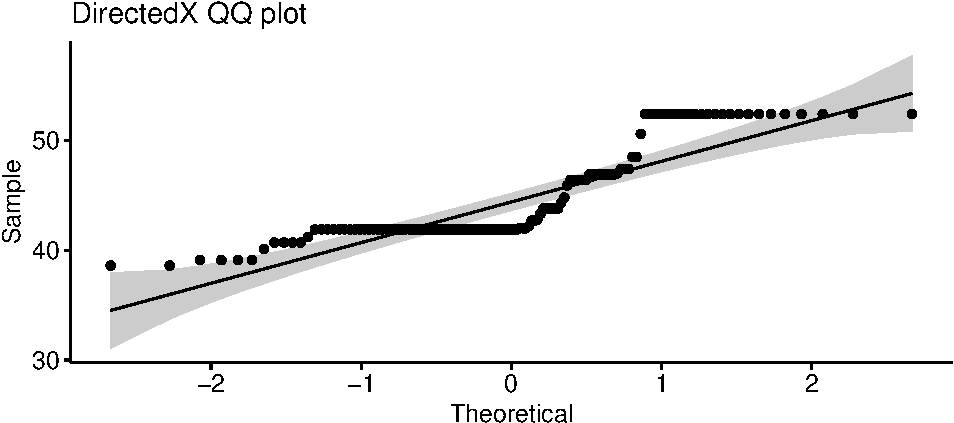
\includegraphics[width=0.85\textwidth]{analyze20-3.pdf}
 \end{center}
 \caption{QQ plot of the data rate observations for the Directional Antenna (tuned version).}
  \label{fig:cf203}
\end{figure}

\newpage

% 
% 
% 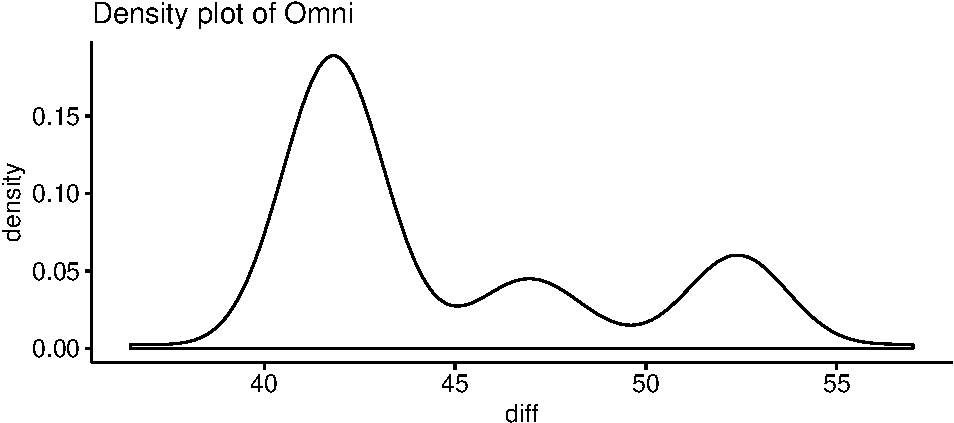
\includegraphics{analyze23-1.pdf}
% 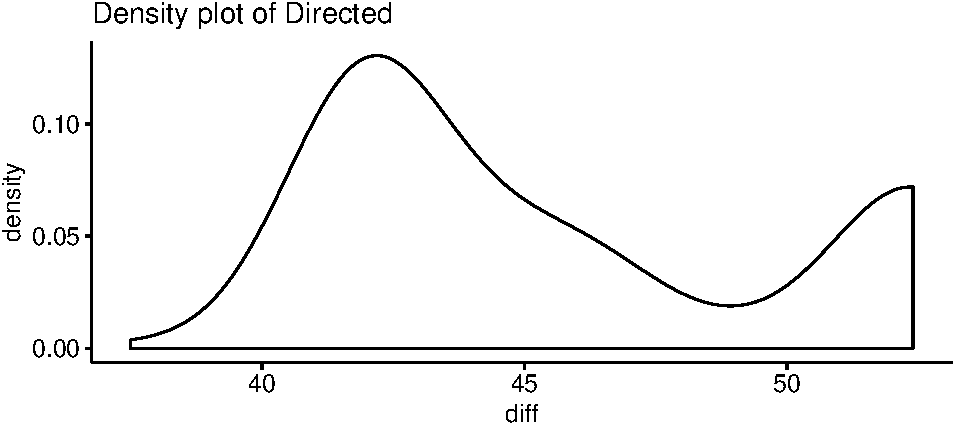
\includegraphics{analyze23-2.pdf}
% 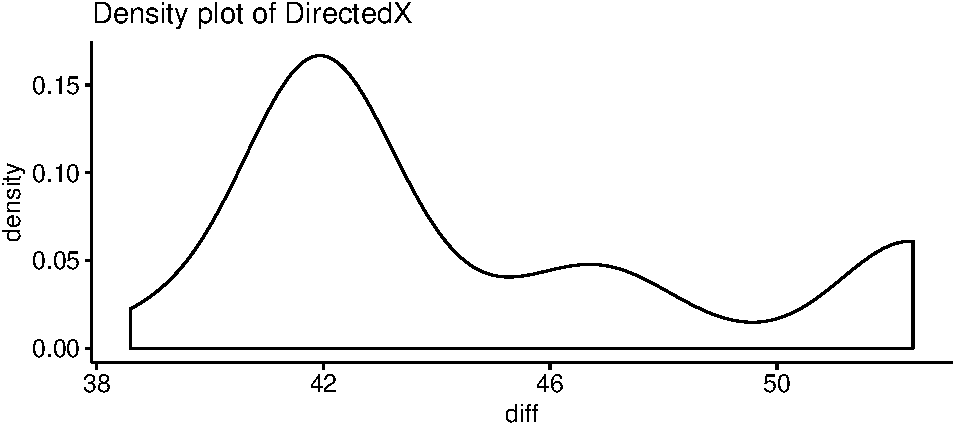
\includegraphics{analyze23-3.pdf}


\begin{figure}[!htbp]
 \begin{center}
  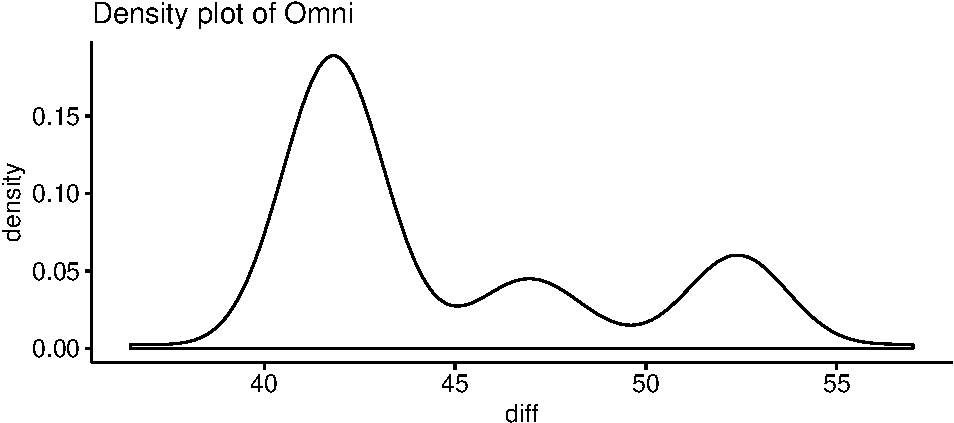
\includegraphics[width=0.85\textwidth]{analyze23-1.pdf}
 \end{center}
 \caption{Density plot of the data rate observations for the Omnidirectional Antenna.}
  \label{fig:cf231}
\end{figure}

\begin{figure}[!htbp]
 \begin{center}
  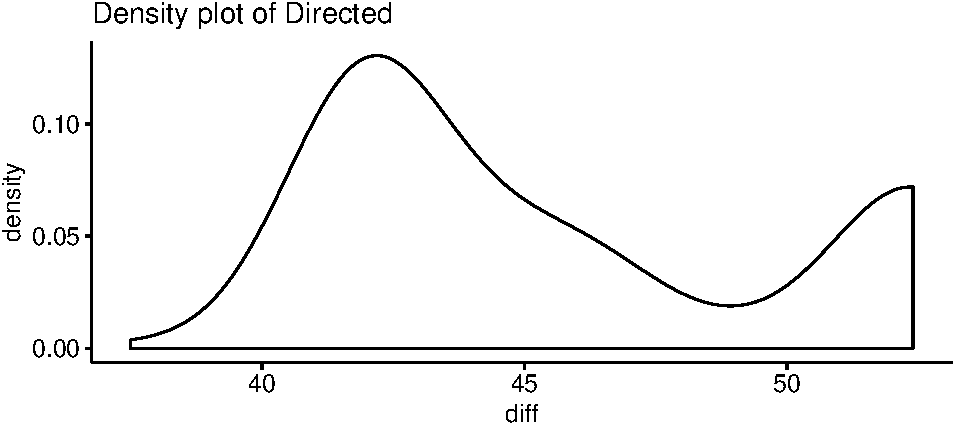
\includegraphics[width=0.85\textwidth]{analyze23-2.pdf}
 \end{center}
\caption{Density plot of the data rate observations for the Directional Antenna.}
  \label{fig:cf232}
\end{figure}

\begin{figure}[!htbp]
 \begin{center}
  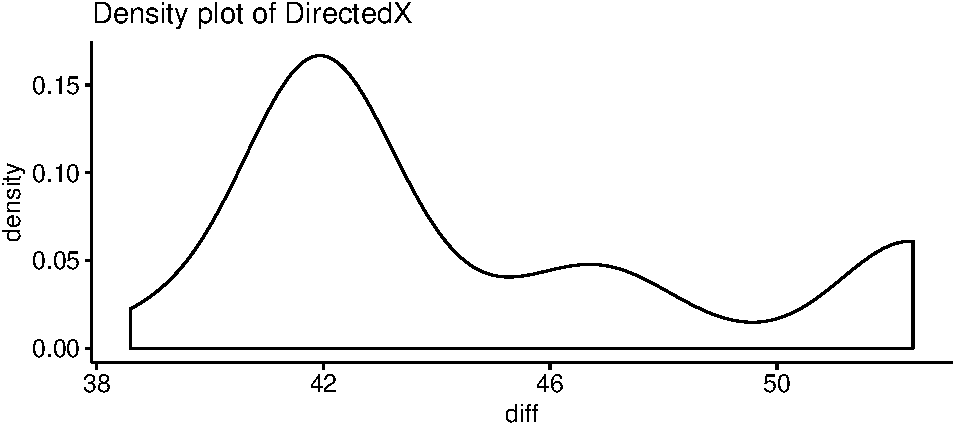
\includegraphics[width=0.85\textwidth]{analyze23-3.pdf}
 \end{center}
 \caption{Density plot of the data rate observations for the Directional Antenna (tuned version).}
  \label{fig:cf233}
\end{figure}

\newpage



% 
% 
% 
% 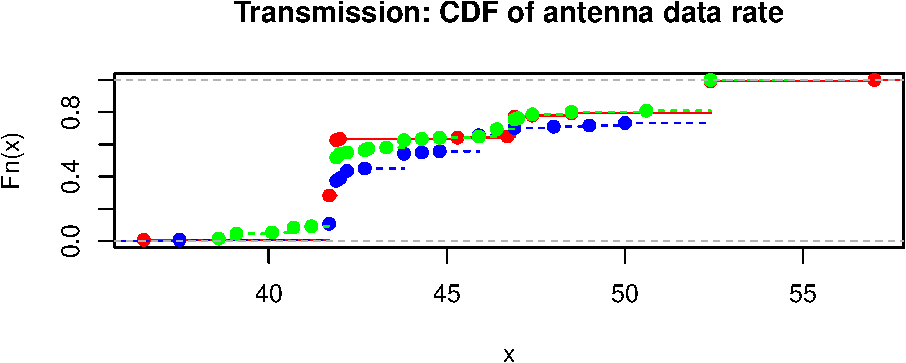
\includegraphics{analyze26-1.pdf}
% 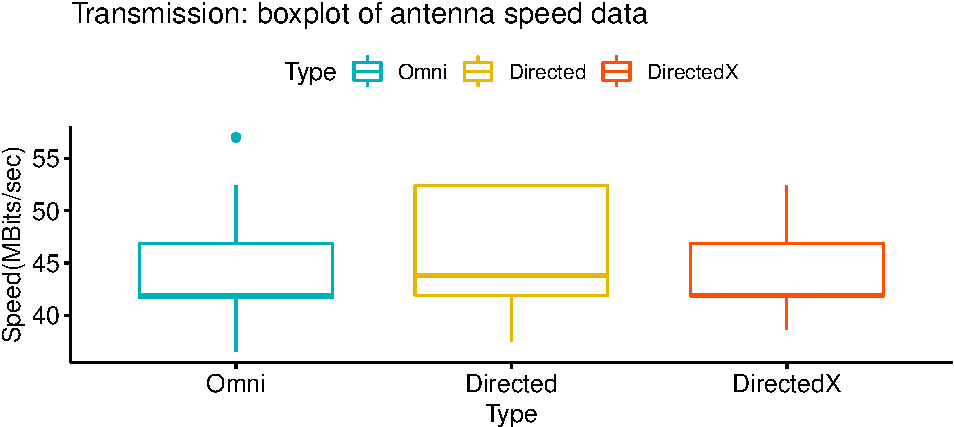
\includegraphics{analyze26-2.pdf}
% 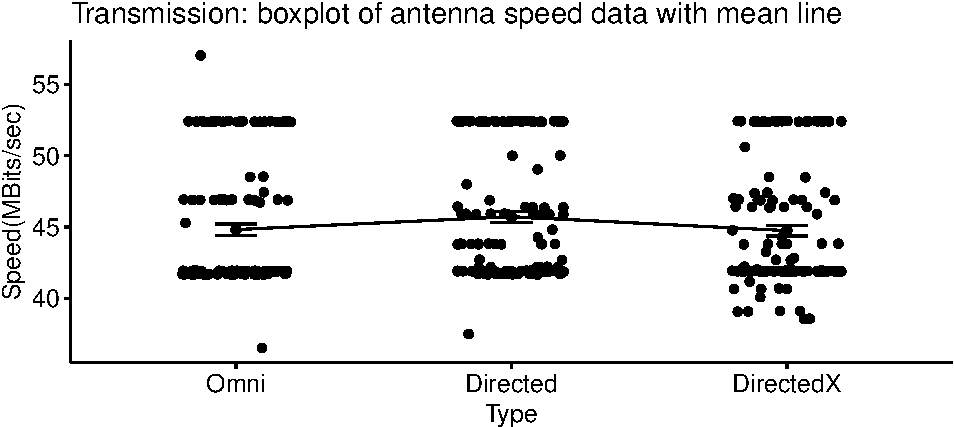
\includegraphics{analyze26-3.pdf}



\begin{figure}[!htbp]
 \begin{center}
  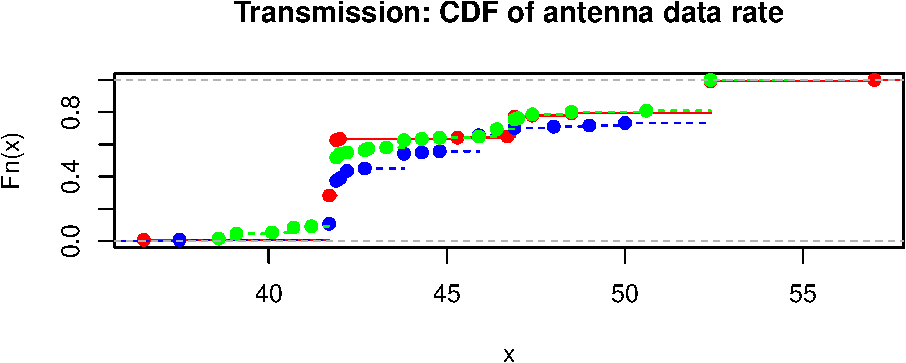
\includegraphics[width=0.85\textwidth]{analyze26-1.pdf}
 \end{center}
 \caption{Cumulative Distribution Function for the data rate observations.}
  \label{fig:cf261}
\end{figure}

\begin{figure}[!htbp]
 \begin{center}
  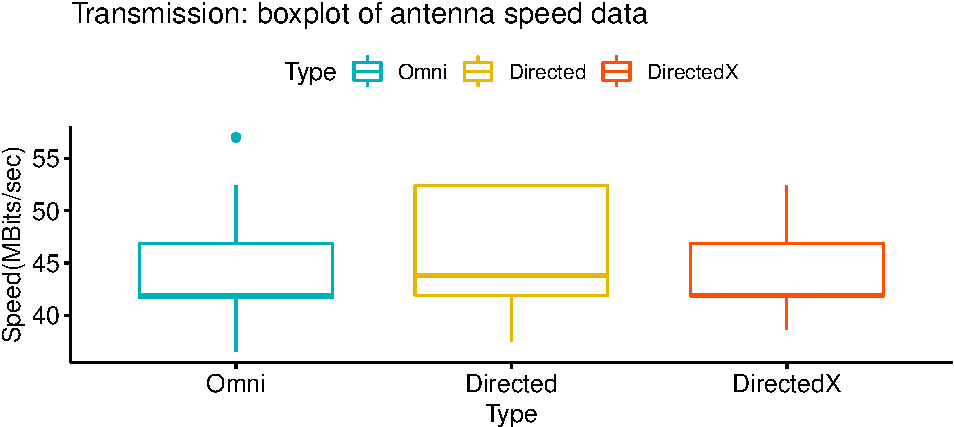
\includegraphics[width=0.85\textwidth]{analyze26-2.pdf}
 \end{center}
 \caption{Boxplot for the data rate observations.}
  \label{fig:cf262}
\end{figure}

\begin{figure}[!htbp]
 \begin{center}
  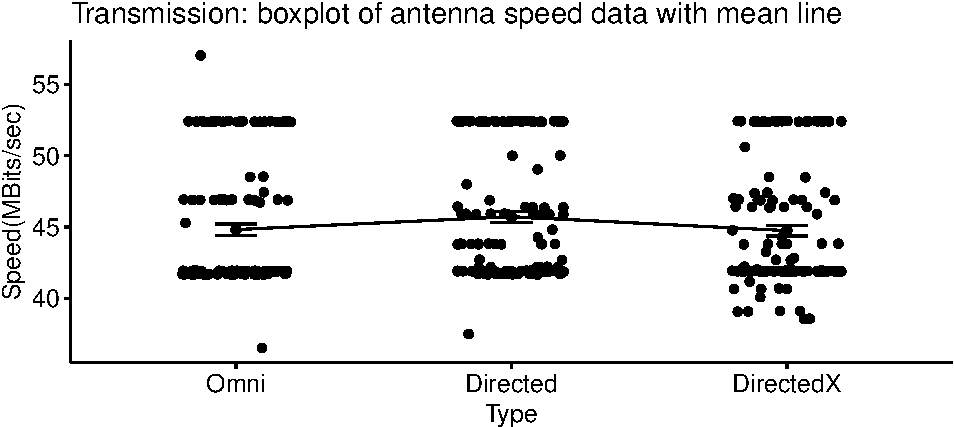
\includegraphics[width=0.85\textwidth]{analyze26-3.pdf}
 \end{center}
 \caption{Boxplot for the data rate observations with the mean line connected.}
  \label{fig:cf263}
\end{figure}

\newpage



\section{R Codes and Results for the Statistical Tests on the Transmission Data}\label{rtrans}

\begin{Shaded}
\begin{Highlighting}[]
\CommentTok{# Testing if the means are same with Welch Two Sample t-test}
\CommentTok{# H0: True difference in means is equal to 0}
\CommentTok{# H1: True difference in means is not equal to 0}
\CommentTok{# If the p-value of the test is less than the significance}
\CommentTok{# level alpha = 0.05.}
\CommentTok{# We reject the Null Hypothesis that: }
\CommentTok{# The means do not have statistically significant difference}
\KeywordTok{t.test}\NormalTok{(Omni,Directed, }\DataTypeTok{alternative =} \StringTok{"two.sided"}\NormalTok{)}
\end{Highlighting}
\end{Shaded}

\begin{verbatim}
##  Welch Two Sample t-test
## data:  Omni and Directed
## t = -1.6488, df = 260, p-value = 0.1004
## alternative hypothesis: true difference in means is not equal to 0
## 95 percent confidence interval:
##  -1.9865682  0.1758812
## sample estimates:
## mean of x mean of y 
##  44.81985  45.72519
\end{verbatim}

\begin{Shaded}
\begin{Highlighting}[]
\KeywordTok{t.test}\NormalTok{(Directed,DirectedX, }\DataTypeTok{alternative =} \StringTok{"two.sided"}\NormalTok{)}
\end{Highlighting}
\end{Shaded}

\begin{verbatim}
##  Welch Two Sample t-test
## data:  Directed and DirectedX
## t = 1.8055, df = 259.73, p-value = 0.07215
## alternative hypothesis: true difference in means is not equal to 0
## 95 percent confidence interval:
##  -0.08854895  2.04274743
## sample estimates:
## mean of x mean of y 
##  45.72519  44.74809
\end{verbatim}

\begin{Shaded}
\begin{Highlighting}[]
\KeywordTok{t.test}\NormalTok{(Omni,DirectedX, }\DataTypeTok{alternative =} \StringTok{"two.sided"}\NormalTok{)}
\end{Highlighting}
\end{Shaded}

\begin{verbatim}
##  Welch Two Sample t-test
## data:  Omni and DirectedX
## t = 0.13278, df = 259.77, p-value = 0.8945
## alternative hypothesis: true difference in means is not equal to 0
## 95 percent confidence interval:
##  -0.9923951  1.1359066
## sample estimates:
## mean of x mean of y 
##  44.81985  44.74809
\end{verbatim}

\pagebreak


\begin{Shaded}
\begin{Highlighting}[]
\CommentTok{# Testing if the data are coming from the same distribution with }
\CommentTok{# Two-sample Kolmogorov-Smirnov test}
\CommentTok{# H0: Two distributions are same}
\CommentTok{# H1: Two distributions are not same}
\CommentTok{# If the p-value of the test is less than the significance}
\CommentTok{# level alpha = 0.05.}
\CommentTok{# We reject the Null Hypothesis that two groups are coming} 
\CommentTok{# from the same dist.}
\KeywordTok{ks.test}\NormalTok{(Omni,Directed, }\DataTypeTok{alternative =} \StringTok{"two.sided"}\NormalTok{)}
\end{Highlighting}
\end{Shaded}
% 
% \begin{verbatim}
% ## Warning in ks.test(Omni, Directed, alternative = "two.sided"): p-value will
% ## be approximate in the presence of ties
% \end{verbatim}

\begin{verbatim}
## 
##  Two-sample Kolmogorov-Smirnov test
## 
## data:  Omni and Directed
## D = 0.25191, p-value = 0.0004906
## alternative hypothesis: two-sided
\end{verbatim}

\begin{Shaded}
\begin{Highlighting}[]
\KeywordTok{ks.test}\NormalTok{(Directed,DirectedX, }\DataTypeTok{alternative =} \StringTok{"two.sided"}\NormalTok{)}
\end{Highlighting}
\end{Shaded}
% 
% \begin{verbatim}
% ## Warning in ks.test(Directed, DirectedX, alternative = "two.sided"): p-value
% ## will be approximate in the presence of ties
% \end{verbatim}

\begin{verbatim}
## 
##  Two-sample Kolmogorov-Smirnov test
## 
## data:  Directed and DirectedX
## D = 0.15267, p-value = 0.09438
## alternative hypothesis: two-sided
\end{verbatim}

\begin{Shaded}
\begin{Highlighting}[]
\KeywordTok{ks.test}\NormalTok{(Omni,DirectedX, }\DataTypeTok{alternative =} \StringTok{"two.sided"}\NormalTok{)}
\end{Highlighting}
\end{Shaded}
% 
% \begin{verbatim}
% ## Warning in ks.test(Omni, DirectedX, alternative = "two.sided"): p-value
% ## will be approximate in the presence of ties
% \end{verbatim}

\begin{verbatim}
## 
##  Two-sample Kolmogorov-Smirnov test
## 
## data:  Omni and DirectedX
## D = 0.19084, p-value = 0.01694
## alternative hypothesis: two-sided
\end{verbatim}

 
